% =========================================================================
% SENDA2 and 3D loading — educational guide 2 (LATTIMEX repository, version 1.1.0)
% SPDX-License-Identifier: CC-BY-4.0
% Build: pdflatex senda2_guide_en && bibtex senda2_guide_en && pdflatex senda2_guide_en && pdflatex senda2_guide_en
% Figure data and number macros in datos2/ (generated by the author from the raw data).
% Translation of guia_senda2.tex. It does not replace senda_guide_en.tex (version 1.0.0), kept unchanged.
% =========================================================================
\documentclass[11pt,a4paper]{article}

\usepackage[T1]{fontenc}
\usepackage{lmodern}
\usepackage[english]{babel}
\usepackage[margin=2.4cm]{geometry}
\usepackage{microtype}
\usepackage{amsmath,amssymb}
\usepackage{booktabs}
\usepackage{array}
\usepackage{graphicx}
\usepackage{float}
\usepackage[font=small,labelfont=bf]{caption}
\usepackage{enumitem}
\usepackage[dvipsnames]{xcolor}
\usepackage{tikz}
\usetikzlibrary{arrows.meta,positioning,calc,shapes.geometric}
\usepackage{pgfplots}
\pgfplotsset{compat=1.18}
\usepackage[most]{tcolorbox}
\usepackage{algorithm}
\usepackage{algpseudocode}
\usepackage{url}
\usepackage[colorlinks=true,linkcolor=MidnightBlue,citecolor=OliveGreen,urlcolor=MidnightBlue]{hyperref}

\algrenewcommand\algorithmicrequire{\textbf{Input:}}
\algrenewcommand\algorithmicensure{\textbf{Output:}}

\definecolor{sendaink}{RGB}{19,34,31}
\definecolor{sendared}{RGB}{210,75,50}
\definecolor{sendagreen}{RGB}{11,131,96}
\newtcolorbox{ideaclave}[1][]{enhanced,breakable,colback=sendagreen!6,colframe=sendagreen!70!black,
  fonttitle=\bfseries,title={Key idea#1},left=6pt,right=6pt,top=4pt,bottom=4pt}
\newtcolorbox{ejemplo}[1][]{enhanced,breakable,colback=MidnightBlue!4,colframe=MidnightBlue!70,
  fonttitle=\bfseries,title={Worked example#1},left=6pt,right=6pt,top=4pt,bottom=4pt}
\newtcolorbox{leccion}[1][]{enhanced,breakable,colback=sendared!6,colframe=sendared!85!black,
  fonttitle=\bfseries,title={Methodological lesson#1},left=6pt,right=6pt,top=4pt,bottom=4pt}
\newtcolorbox{reproducir}[1][]{enhanced,breakable,colback=gray!6,colframe=gray!60!black,
  fonttitle=\bfseries,title={To reproduce#1},left=6pt,right=6pt,top=4pt,bottom=4pt}

\newcommand{\senda}{SENDA}
\newcommand{\sendados}{SENDA2}
\newcommand{\pp}{\,pp}
\newcommand{\tsl}[1]{\texttt{\small #1}}

% generado por tools/datos_guia2.py
\newcommand{\FiloABE}{0.053}
\newcommand{\FiloX}{0.72}
\newcommand{\HgsABE}{0.006}
\newcommand{\HgsX}{1.40}
\newcommand{\NABEtres}{55}
\newcommand{\ProdInvalidosMotor}{9}
\newcommand{\ProdRechazoMotor}{70.8}
\newcommand{\ProdRechazoPtresL}{14.6}
\newcommand{\ProdRechazoPtresLq}{3.8}
\newcommand{\SendaDosABE}{0.074}
\newcommand{\SendaDosGanaHgsX}{7}
\newcommand{\SendaDosX}{1.74}

% generado por tools/macros_motor.py
\newcommand{\AochoExGap}{+26.4\,\%}
\newcommand{\AochoExValid}{145/285}
\newcommand{\AochoProdLoValid}{pendiente}
\newcommand{\AochoProdRelaxed}{pendiente}
\newcommand{\AochoProdValid}{pendiente}
\newcommand{\AochoUpGap}{pendiente}
\newcommand{\AochoUpGapEasy}{pendiente}
\newcommand{\AochoUpGapHard}{pendiente}
\newcommand{\AochoUpValid}{pendiente}
\newcommand{\HashAocho}{pendiente}
\newcommand{\HashNivelUno}{1944dc5be91d}
\newcommand{\HashNivelUnoP}{e2bde2f206bd}
\newcommand{\HashRondaDos}{8dfb1d575211}
\newcommand{\HashSdosRtres}{ab706daaaabf}
\newcommand{\ReproABE}{0.086}
\newcommand{\ReproX}{1.77}
\newcommand{\ReproXParalelo}{1.96}
\newcommand{\VerifConcuerda}{2\,436}


\title{\textbf{SENDA2 and three-dimensional loading:\\ from classic routing to the integrated problem, measured honestly}\\[0.4em]
\large Second educational guide to the LATTIMEX engine (version 1.1.0): what changed, how it was measured\\ and how to try it on your computer}
\author{Erick Martínez\\
\small LATTIMEX · independent research · Querétaro, Mexico\\
\small \texttt{contacto@lattimex.com} · \texttt{https://lattimex.com}}
\date{October 2026}

\hypersetup{
  pdftitle={SENDA2 and three-dimensional loading: LATTIMEX educational guide 2},
  pdfauthor={Erick Martínez (LATTIMEX)},
  pdfsubject={Vehicle routing with three-dimensional loading (3L-CVRP)},
  pdfkeywords={CVRP, 3L-CVRP, ALNS, 3D packing, unloading order, reproducible evaluation}
}

\makeatletter
\def\ps@licenciaguia{%
  \let\@oddhead\@empty
  \let\@evenhead\@empty
  \def\@oddfoot{\vtop{\offinterlineskip%
    \hbox to\textwidth{\hfil\thepage\hfil}%
    \vskip5pt
    \hbox to\textwidth{\hfil\scriptsize\textcopyright{} 2026 Erick Martínez (LATTIMEX).
      CC BY 4.0: \url{https://creativecommons.org/licenses/by/4.0/}\hfil}}}%
  \let\@evenfoot\@oddfoot
}
\makeatother

\begin{document}
\maketitle
\thispagestyle{licenciaguia}

\begin{abstract}
\noindent\textbf{In a nutshell.} The first guide opened \senda, the LATTIMEX routing core, and measured
it on the classic problem. This second guide reports the advance: a better core (\sendados), a new
three-dimensional packer (P3L) and their integration in engine 1.1.0, which is open source (MIT). Like
the first one, it explains every piece from scratch and gives as much room to \emph{how} things were
measured as to the results, including our own mistakes that the measurement uncovered.

\smallskip
\noindent \sendados{} adds three changes to the adaptive large neighbourhood search of \senda: a
cached repair, discarding repairs that do not fit, and a 0.02\,s cap on polishing each new best. In a
single session, with the same clock and independent verification, it is +0.33\pp{} behind HGS-CVRP on
41 X instances at 4\,s (\SendaDosX\,\% versus \HgsX\,\%; FILO2, \FiloX\,\%) and +0.07\pp{} on A/B/E at
2\,s with a fixed fleet; the first guide reported a distance of about 2.6\pp{} on X. For loading, we
built a harness against the published optima of Tamke et al.\ (2026) and the validator of Krebs and
Ehmke (2023). It revealed that the 1.0.0 packer rejected 34\,\% to 61\,\% of routes that do fit and
allowed a later box on top of an earlier one. P3L lowers that rejection to 24--36\,\% and, with the
strict checker, the engine no longer returns packings that violate the unloading order. A routing
search that checks the load at every step (R3L) achieves 285 of 285 valid solutions on the 19 Gendreau
instances, at +6.9\,\% distance from Tamke's solutions (which ran up to 8 hours per instance). R3L does
not scale to 300 deliveries; the document explains why and what remains open.
\end{abstract}

\noindent\textbf{Keywords:} vehicle routing; CVRP; 3L-CVRP; ALNS; three-dimensional packing; unloading
order (LIFO); reproducible evaluation; optimization teaching.

\tableofcontents
\newpage

% =========================================================================
\section*{How to read this document}
\addcontentsline{toc}{section}{How to read this document}

This guide continues the first one (\emph{SENDA: vehicle routing with single-trajectory search,
explained and honestly measured}, September 30, 2026, \tsl{paper/senda\_guide\_en.pdf}). It does not
replace it: the first remains the reference to understand \senda{} piece by piece (construction,
granular local search, ALNS, segment moves, portfolio) and the basics of a fair comparison. Here that
knowledge is assumed and only what is new is explained.

\begin{itemize}[leftmargin=1.5em]
\item Section~\ref{sec:sendados} presents \sendados, how we got there and how it compares with
HGS-CVRP and FILO2 on the classic problem.
\item Section~\ref{sec:carga} introduces the problem with three-dimensional loading, explains how to
measure a packer without fooling yourself and presents P3L.
\item Section~\ref{sec:integracion} joins routing and packing: why a good packer is not enough, what
R3L is and what engine 1.1.0 achieves.
\item Section~\ref{sec:pruebalo} explains how to use the full engine or each piece on its own.
\end{itemize}

The boxes have the same four roles as in the first guide:

\begin{ideaclave}
Summarizes the concept not to forget.
\end{ideaclave}
\begin{ejemplo}
Works out a small calculation, step by step, with concrete numbers.
\end{ejemplo}
\begin{leccion}
Describes a possible mistake, or one that actually happened in this project, and how to avoid it.
\end{leccion}
\begin{reproducir}
Gives the SHA-256 fingerprints of the artifacts behind a figure and how to repeat the measurement.
\end{reproducir}

\paragraph{About this edition.} It accompanies version 1.1.0 of the public LATTIMEX repository. The
repository contains the engine and this guide; it does not contain the comparison programs (HGS-CVRP,
FILO2, Krebs's validator, the exact CP-SAT model) nor the campaign scripts. They are described here so
that the comparison is transparent; raw data, contracts and logs are kept in the author's archive and
each figure cites the fingerprint of the artifact behind it.

% =========================================================================
\section{Introduction}
\label{sec:intro}

The first guide ended with three open tasks: give the search more effective time on large instances,
measure the core on the integrated problem with three-dimensional loading, and widen the benchmark.
This guide reports what happened with the first two.

The short answer has three parts:

\begin{enumerate}[leftmargin=1.5em]
\item \textbf{\sendados.} Three small changes to the ALNS of \senda{} close most of the distance to
HGS-CVRP on the X instances: from about 2.6 to 0.33 gap points at 4\,s. The path included our own
measurement error and a hypothesis (the \emph{k-medoids} seed) that ablation ruled out.
\item \textbf{P3L and the strict checker.} Measuring the 1.0.0 packer against routes \emph{known} to
fit showed that it rejected half of them and that its unloading-order rule had a gap. P3L is a new
packer with the standard semantics; the strict checker guarantees the engine never returns an invalid
packing.
\item \textbf{Integration.} A good packer is not enough: if routing does not know what fits, it
proposes impossible routes. R3L, a routing search that asks the packer at every step, solves validity
on small instances; at product scale the engine uses P3L inside \sendados{} routing and warns when it
cannot keep the unloading order.
\end{enumerate}

\begin{ideaclave}
Every advance in this guide started with a measurement that contradicted what we believed. Version
1.0.0 was not worse than advertised at routing, but it was at loading: with unloading order it returned
plans that violated it. Measuring against known optima with an independent judge is what made it
visible.
\end{ideaclave}

% =========================================================================
\section{\sendados: the routing core}
\label{sec:sendados}

\subsection{What changes with respect to \senda}

\senda{} (first guide, Sections 3 to 7) follows a single trajectory per run: it constructs, improves
with granular local search, restructures with an ALNS that destroys part of the solution and repairs
it, polishes each new best and splits its time among two or three configurations. \sendados{} keeps all
of that and changes three things inside the ALNS:

\begin{enumerate}[leftmargin=1.5em,label=(\alph*)]
\item \textbf{Cached regret repair.} When reinserting the removed customers, the repair of \senda{}
recomputes, for each customer and at every step, its best position in all routes. \sendados{} keeps a
single candidate insertion per route for each customer (the cheapest among the positions next to its
granular neighbours) and, after each insertion, only recomputes the route that changed. Each repair
costs much less and the ALNS does more iterations in the same time.
\item \textbf{Discarding failed repairs.} With a fixed fleet and no penalty, if the repair cannot fit
every customer without exceeding capacity, \sendados{} discards the candidate (and penalizes the
weights of the operators that produced it) instead of accepting it infeasible.
\item \textbf{Polish cap.} Each time a new best appears, \senda{} polishes it with local search until
it no longer improves. \sendados{} limits that polishing to $\min(0.02\text{\,s},\,0.20\cdot t_{\text{rem}})$,
where $t_{\text{rem}}$ is the remaining time.
\end{enumerate}

\begin{ejemplo}[: how much time the polish cap frees]
On X at 4\,s, each solver has 80\,\% of the clock: 3.2\,s. In the measurement before \sendados, polishing
each new best used on average about 1.9 of those 3.2\,s, almost 60\,\%. With the 0.02\,s cap, a trial that
finds 40 new bests spends at most $40 \times 0.02 = 0.8$\,s polishing, and the rest goes back to the
ALNS. In the confirmation (Section~\ref{sec:confirmacion}), mean iterations on X went from 654 to
1\,402 per trial and the gap dropped by 0.59 points.
\end{ejemplo}

\subsection{How we got there: two useful mistakes}

\begin{leccion}[: the degraded control]
The first candidate, called \emph{KM-R1}, seeded the initial solution with $k$-medoids and destroyed by
medoids. Its first comparison against \senda{} showed a large advantage. On repeating it we found that
the control (\senda) had run at half its normal iterations: another session, another machine load.
Repeated with all three arms in the same session and with a \emph{speed sentinel} (the control's
iterations must match those of a reference run), the advantage was still real but smaller. Rule:
\textbf{all arms in the same session, in rotated order, with a speed sentinel}; never against a number
from another session.
\end{leccion}

\begin{leccion}[: the name that ablation removed]
With the advantage confirmed, it was tempting to credit the $k$-medoids. Ablation (removing one piece
at a time, in the same session) said otherwise: removing the seed or the medoid destruction changed
nothing; removing the cached repair cost 0.87 points on X, and the polish cap explained most of the
rest. The candidate was simplified to those pieces and lost the name ``SENDA-KM'': it is called
\sendados. Moreover, the 0.02\,s cap was chosen by looking at one round's data, so its figure could not
be published without repeating it with new seeds (Section~\ref{sec:confirmacion}).
\end{leccion}

\subsection{Results against HGS-CVRP and FILO2}
\label{sec:confirmacion}

\paragraph{Design.} As in the first guide: 60 A/B/E instances with a fixed fleet at 2\,s and 41 X
instances with a free fleet at 4\,s; 80\,\% of the clock as internal budget for every solver; one
thread; distances rounded to integers (CVRPLIB convention); independent verification of coverage,
capacity, fleet and cost. HGS-CVRP~\cite{vidal2022hgs} and FILO2~\cite{accorsi2023} were compiled from
their official sources. The main table is a session with all three solvers and never-used seeds
(3000--3900); the H1-C confirmation, with other new seeds (2000--2900), repeats the comparison with
HGS.

\begin{table}[H]
\centering
\caption{Mean gap to the best known solution (BKS). Same session, same clock. On A/B/E we average the
\NABEtres{} instances where all three solvers respected the fleet in every run (FILO2 has no
fixed-fleet option and used one extra route on 5 instances).}
\label{tab:cvrp}
\begin{tabular}{lrrr}
\toprule
& \sendados & HGS-CVRP & FILO2 \\
\midrule
X, 41 instances, 4\,s, 5 seeds & \SendaDosX\,\% & \HgsX\,\% & \textbf{\FiloX\,\%} \\
A/B/E, \NABEtres{} instances, 2\,s, 10 seeds & \SendaDosABE\,\% & \textbf{\HgsABE\,\%} & \FiloABE\,\% \\
\bottomrule
\end{tabular}
\end{table}

\paragraph{Paired comparisons.} Per instance, $\Delta$ = gap of \sendados{} minus gap of the other
solver (bootstrap 95\,\% CI; Wilcoxon test):
\begin{itemize}[leftmargin=1.5em]
\item \textbf{Against HGS, on X:} $+0.33$\pp{} [0.21, 0.45], $p = 3\cdot10^{-6}$; \sendados{} is better
on \SendaDosGanaHgsX{} of 41 instances. The H1-C confirmation gives $+0.34$\pp{} with \sendados{} and
$+0.28$\pp{} [0.13, 0.42] with a variant that kept the discarded pieces.
\item \textbf{Against HGS, on A/B/E:} $+0.068$\pp{} [0.033, 0.111]; tie on 36 instances and HGS is
better on 19.
\item \textbf{Against FILO2:} on X, $+1.02$\pp{} [0.85, 1.17], and FILO2 wins on 40 of 41; on A/B/E no
clear difference was detected ($+0.021$\pp{}, CI crossing zero).
\end{itemize}

\begin{figure}[H]
\centering
\begin{tikzpicture}
\begin{axis}[width=0.92\textwidth,height=6.2cm,xlabel={customers ($n$)},ylabel={mean gap (\%)},
  legend style={at={(0.5,1.03)},anchor=south,legend columns=3,draw=none},legend cell align=left,
  grid=major,grid style={gray!20},ymin=0]
\addplot[only marks,mark=*,mark size=1.5pt,sendared] table[x=n,y=senda2]{datos2/x_senda2.dat};\addlegendentry{\sendados}
\addplot[only marks,mark=square*,mark size=1.5pt,MidnightBlue] table[x=n,y=hgs]{datos2/x_senda2.dat};\addlegendentry{HGS-CVRP}
\addplot[only marks,mark=triangle*,mark size=1.8pt,sendagreen] table[x=n,y=filo2]{datos2/x_senda2.dat};\addlegendentry{FILO2}
\end{axis}
\end{tikzpicture}
\caption{Mean gap per X instance at 4\,s (5 seeds per solver, same session). FILO2's advantage grows
with instance size.}
\label{fig:x}
\end{figure}

\paragraph{Against \senda.} The first guide reported, on another machine, 4.119\,\% on X versus
1.450\,\% for HGS. To avoid mixing sessions, the honest comparison uses HGS as a common anchor: in an
October session, \senda{} was $+2.64$\pp{} behind HGS on X (4.05\,\% versus 1.41\,\%); \sendados{} is
$+0.33$\pp{} behind. On A/B/E, from $+0.094$ to $+0.068$\pp.

\begin{ideaclave}
The honest claim is not ``state of the art'': FILO2 is clearly stronger on large instances with a short
clock, and HGS is still better on average. \sendados{} is a core of about 2\,200 lines, single
trajectory, that respects a fixed fleet and stays close to HGS. Its value lies in being simple,
auditable and carefully measured.
\end{ideaclave}

\begin{reproducir}
Session with all three solvers: \tsl{raw\_trials.jsonl} \tsl{ef823740c317\ldots}, contract
\tsl{906e37b0ab29\ldots}. H1-C confirmation: \tsl{2ac424ad3411\ldots}. With the repository:
\tsl{python -m lattimex cvrp INSTANCE.vrp --time 4} (X) or \tsl{--time 2 --fleet fixed} (A/B/E) splits
the time and picks configurations as in the measurement. Repeated on the same benchmark with the
published binary, one run at a time, it gave \ReproX\,\% on X (41 instances, 1 seed) and \ReproABE\,\%
on A/B/E (60 instances, 2 seeds), within seed-to-seed variation. \textbf{Run one instance at a time}:
with six processes in parallel on the same machine the X gap rose to \ReproXParalelo\,\%, because each
process did fewer iterations.
\end{reproducir}

\subsection{\sendados{} inside the engine}
\label{sec:motor-ruteo}

The engine does not call the core the way the benchmark does: it splits the budget among routing,
packing and re-optimization, uses an exact fleet and runs a portfolio of configurations on two threads.
Measured that way (107 instances, 3 seeds, same session), \sendados{} versus \senda:

\begin{itemize}[leftmargin=1.5em]
\item A/B/E: $-0.036$\,\% distance [$-0.068$, $-0.009$], $p=0.02$.
\item X: the result depends on how many customers each route serves (Spearman $\rho=-0.65$). With 12
or more customers per route, $-0.89$\,\% (wins on 14 of 16); with fewer than 6, $+2.99$\,\% (loses on 9
of 12).
\end{itemize}

Real LATTIMEX routes are long (30 to 75 deliveries per vehicle), so engine 1.1.0 uses \sendados{} by
default and falls back to the 1.0.0 core when there are fewer than 6 deliveries per vehicle. The rule
was set with the same data that motivate it; it is an engineering decision, not a confirmed figure.

The same round found a risk in the exact-fleet constructor: when the load fills between 92.5\,\% and
99.7\,\% of total capacity, it could not split it into $k$ vehicles and the engine rejected the order (11
of 41 X instances). Engine 1.1.0 adds a fallback that assigns accepting overload and removes it with
local search; it solved all 11 in under half a second.

% =========================================================================
\section{Loading: measuring and building a packer}
\label{sec:carga}

\subsection{The problem with three-dimensional loading}

In the 3L-CVRP~\cite{gendreau2006} each customer orders boxes with length, width, height, weight and a
fragility flag, and each route must fit inside the vehicle's cargo space. We use Gendreau's axes: $x$
is the length (the door is at $x=L$), $y$ the width and $z$ the height; boxes only rotate horizontally.
Besides staying inside and not overlapping, a packing may require:

\begin{itemize}[leftmargin=1.5em]
\item \textbf{Support:} at least 75\,\% of each box's base rests on the floor or on boxes whose top face
is at that height.
\item \textbf{Fragility:} a non-fragile box cannot rest on a fragile one.
\item \textbf{Unloading order (LIFO):} on reaching each customer, its boxes come out without moving
those of later customers.
\end{itemize}

The five standard variants combine these rules:

\begin{table}[H]
\centering
\caption{3L-CVRP variants (Gendreau et al., 2006).}
\label{tab:variantes}
\begin{tabular}{lccc}
\toprule
Variant & Support & Fragility & Unloading order \\
\midrule
loading-only & -- & -- & -- \\
no-support & -- & yes & yes \\
no-fragility & yes & -- & yes \\
no-lifo & yes & yes & -- \\
all-constraints & yes & yes & yes \\
\bottomrule
\end{tabular}
\end{table}

\paragraph{The unloading order, precisely.} Let $e$ be a box of a customer visited \emph{before} the
customer of box $t$. The packing violates the order if $t$ blocks $e$ in one of two ways
(Figure~\ref{fig:lifo}): (i) $t$ is \emph{in front of} $e$, closer to the door, and their projections on
the $y$--$z$ plane touch; or (ii) $t$ is \emph{on top of} $e$ and their projections on the $x$--$y$
plane touch. These are the semantics of the public validator of Krebs and
Ehmke~\cite{krebs2023,krebsvalidator}.

\begin{figure}[H]
\centering
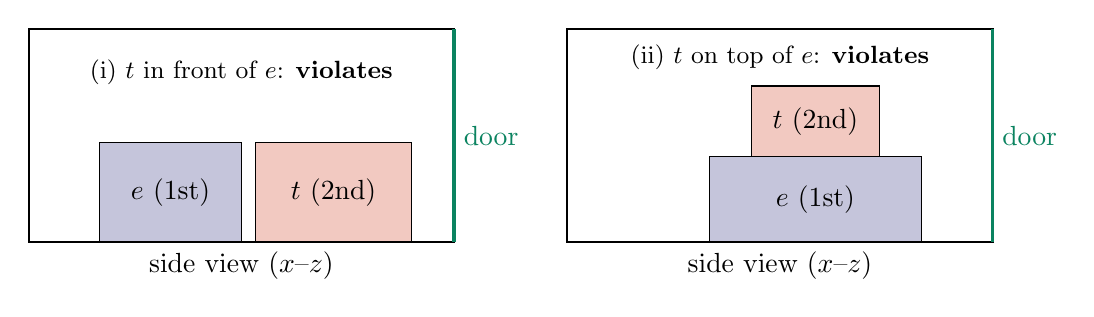
\begin{tikzpicture}[scale=0.9]
  \begin{scope}
    \draw[thick] (0,0) rectangle (6,3); \node[below] at (3,0) {side view ($x$--$z$)};
    \draw[very thick,sendagreen] (6,0) -- (6,3); \node[right,sendagreen] at (6,1.5) {door};
    \filldraw[fill=MidnightBlue!25] (1,0) rectangle (3,1.4); \node at (2,0.7) {$e$ (1st)};
    \filldraw[fill=sendared!30] (3.2,0) rectangle (5.4,1.4); \node at (4.3,0.7) {$t$ (2nd)};
    \node[align=center,font=\small] at (3,2.4) {(i) $t$ in front of $e$: \textbf{violates}};
  \end{scope}
  \begin{scope}[xshift=7.6cm]
    \draw[thick] (0,0) rectangle (6,3); \node[below] at (3,0) {side view ($x$--$z$)};
    \draw[very thick,sendagreen] (6,0) -- (6,3); \node[right,sendagreen] at (6,1.5) {door};
    \filldraw[fill=MidnightBlue!25] (2,0) rectangle (5,1.2); \node at (3.5,0.6) {$e$ (1st)};
    \filldraw[fill=sendared!30] (2.6,1.2) rectangle (4.4,2.2); \node at (3.5,1.7) {$t$ (2nd)};
    \node[align=center,font=\small] at (3,2.6) {(ii) $t$ on top of $e$: \textbf{violates}};
  \end{scope}
\end{tikzpicture}
\caption{The two ways a box $t$ of a later delivery blocks a box $e$ of an earlier delivery. The 1.0.0
packer only forbade the first.}
\label{fig:lifo}
\end{figure}

\subsection{How to measure a packer without fooling yourself}

Measuring a packer looks easy: give it routes and count how many it packs. The trap is that you do not
know how many \emph{should} fit. Given loose routes, any packer looks good; given impossible routes, any
packer looks bad.

\paragraph{Routes known to fit.} Tamke et al.~\cite{tamke2025} solved with an exact branch-and-cut the
19 classic Gendreau instances with up to 50 customers, in all five variants, and published their
solutions with the packing of each route~\cite{tamkerepo}. Each of those 648 routes fits: its packing
exists and the validator approves it. If a packer rejects one of them, it is a \textbf{false
rejection}, with no ambiguity. We call this test \emph{level 1}.

\paragraph{An independent judge.} Every accepted packing is checked with Krebs's validator, which is
not part of the engine. Before using it as a judge we checked that it judges correctly: it approves
Tamke's 95 solutions (19 instances $\times$ 5 variants), rejects the 76 solutions of loose variants
evaluated with all constraints, and rejects the 19 cases with a forced overlap.

\begin{leccion}[: the 2.4\,\% that did not measure what it seemed]
In July we had reported that the engine's packer rejected only 2.4\,\% of routes. That measurement used
routes from another heuristic built with all constraints and tested them on the loosest variant: they
were loose routes. With the optimal routes, which are tight, rejection was 34 to 64\,\%. A quality
figure only means something together with the benchmark it was measured on.
\end{leccion}

\subsection{What the measurement found in version 1.0.0}

\begin{itemize}[leftmargin=1.5em]
\item \textbf{High false rejection:} between 36\,\% (loading-only) and 64\,\% (all-constraints) of the
optimal routes, growing with route size: with 9 to 12 boxes, 47 of 49 rejected. With 1\,024 restarts
instead of the usual ones, all-constraints only dropped from 64\,\% to 60\,\%: the limit was the
placement algorithm, not the effort.
\item \textbf{A gap in the unloading order:} the packer forbade case (i) of Figure~\ref{fig:lifo} but
not (ii). Krebs rejected 27 packings the engine considered valid.
\item \textbf{In the full engine,} with all constraints, 1 of 57 runs was valid: when a route did not
fit, the engine silently relaxed the unloading order.
\end{itemize}

\subsection{P3L}

P3L (\tsl{native/p3l.cpp}) packs one route in one container with the semantics of
Figure~\ref{fig:lifo}:

\begin{enumerate}[leftmargin=1.5em]
\item \textbf{Loading sequence.} With unloading order, boxes are loaded from the last customer to the
first; within each customer, by volume, base area, height or longest side.
\item \textbf{Gravity placement.} For each box, candidate positions in $x$ and $y$ are generated (the
origin, the end of each placed box and the opposite wall) and each one drops until it rests; the first
one by a lexicographic rule wins (for example, smallest $x$, then smallest $z$).
\item \textbf{Beam search} over the sequence: the best partial sequences are kept according to their
contact with walls and boxes.
\item \textbf{Iterated local search} over the loading sequence and rotations, from several starts, until
everything is placed or the cap runs out (50\,ms per route in the engine).
\end{enumerate}

\begin{leccion}[: positions that seem enough and are not]
To speed up, it is common to restrict positions to \emph{normal patterns}: the sums of box lengths. It is
correct without support or unloading order, but not with them. An exact CP-SAT model, used as a
reference during development, ``proved'' impossible 5 routes that Tamke had packed. The cause was the
normal patterns; with all integer positions in $x$ and $y$ when there is support, as Tamke does, the 5
routes fit.
\end{leccion}

\paragraph{Results at level 1.} The 13 instances not used to tune P3L, with the frozen candidate
(Table~\ref{tab:nivel1}). The ``P3L + CP-SAT'' column adds the exact model for the routes P3L does not
pack; it lowers rejection almost to zero, but it is not part of the engine: it depends on OR-Tools and
does not finish on routes of 55 or more boxes.

\begin{table}[H]
\centering
\caption{False rejection on Tamke's optimal routes, 13 confirmation instances. No packing accepted by
P3L was rejected by the validator.}
\label{tab:nivel1}
\begin{tabular}{lrrr}
\toprule
Variant & 1.0.0 packer & \textbf{P3L} (engine 1.1.0) & P3L + CP-SAT \\
\midrule
loading-only & 34.1\,\% & 23.9\,\% & 1.1\,\% \\
no-support & 42.2\,\% & 33.3\,\% & 0.0\,\% \\
no-fragility & 57.6\,\% & 32.6\,\% & 0.0\,\% \\
no-lifo & 41.1\,\% & 35.6\,\% & 6.7\,\% \\
all-constraints & 61.3\,\% & 30.1\,\% & 0.0\,\% \\
\bottomrule
\end{tabular}
\end{table}

\paragraph{At product scale.} On 159 routes of 20 to 97 boxes produced by the engine on 12 Querétaro
instances, with all constraints, the 1.0.0 packer rejected at least \ProdRechazoMotor\,\% of the routes
that fit and gave \ProdInvalidosMotor{} invalid packings; P3L with 50\,ms, at least
\ProdRechazoPtresL\,\%, and with 500\,ms, at least \ProdRechazoPtresLq\,\%, with no invalid ones (``at
least'' because there are no optima here: a route counts as feasible if some method packed it). Without
unloading order, both pack all of them.

\paragraph{The strict checker.} Engine 1.1.0 checks every packing with the semantics of
Figure~\ref{fig:lifo} before accepting it, whether it comes from P3L or from the 1.0.0 packer, which is
kept as a fallback because it can turn boxes vertically when allowed. Against Krebs's validator, the
checker agreed on \VerifConcuerda{} of \VerifConcuerda{} packings, including 105 that Krebs rejects.

% =========================================================================
\section{Integration: routing that knows what fits}
\label{sec:integracion}

\subsection{Why a good packer is not enough}

The engine routes with an effective volume capacity, a fraction of the vehicle's volume, and packs
afterwards. If a route does not fit, a \emph{mediation} tries a few changes: reverse it, rotate it or
move a customer to another route. Replacing only the packer with P3L raised valid runs with all
constraints from 1 to 20 of 57, but the gap of the valid ones did not change (+15 to +29\,\%) and the
exact model proved impossible 1\,665 routes that routing had proposed. Routing kept proposing routes
without knowing whether they fit.

\subsection{R3L}

R3L (\tsl{lattimex/engine/r3l.py}) is a ruin-and-recreate routing search in the style of
SISR~\cite{christiaens2020} with simulated annealing~\cite{kirkpatrick1983}, in which every insertion
asks the packer:

\begin{algorithm}[H]
\caption{R3L (outline)}
\begin{algorithmic}[1]
\Require customers, distance matrix, container, variant, maximum fleet $k$, time $T$
\State $S \gets$ rebuild from scratch; if there are \sendados{} routes, also from them, and keep the best
\While{time remains}
  \State $S' \gets$ remove from $S$ strings of nearby customers (SISR)
  \For{each removed customer, in random order or by volume or distance}
    \State try its positions from cheapest to most expensive;
    \State keep the first whose route \textbf{fits} (P3L); open a new route only if there are fewer than $k$
  \EndFor
  \State accept $S'$ with the simulated annealing criterion; keep the best complete solution
\EndWhile
\end{algorithmic}
\end{algorithm}

Three details make it fast. (1) Checks are staged: one greedy P3L pass for every candidate position
(0.3\,ms on small routes) and beam search only for the cheapest position. (2) A cache stores every
verdict; without unloading order the key is the set of customers, because the order does not change the
packing. (3) With unloading order, if a route does not fit it is tried reversed: same distance,
different unloading order.

\begin{ejemplo}[: the reversed route]
A route visits A and then B. A orders a non-fragile box that covers the whole floor; B, a fragile one
of the same size. In the order A, B, B's box (second delivery) must be loaded first, at the back or
below; since it covers the whole floor, it goes below and A's on top: a non-fragile box on a fragile
one, forbidden. In the order B, A, A's box goes below and B's fragile one on top: allowed, and B comes
out first without moving anything. The distance is the same; R3L only has to try the route both ways.
\end{ejemplo}

\subsection{Results against Tamke}

The 19 Gendreau instances, all five variants and three seeds (285 runs per arm), with an ``up to $k$''
fleet ($k$ = available vehicles, as in Tamke). A run is \emph{valid} if Krebs's validator approves
routing and loading in the variant. The gap is the distance against Tamke's solution.

\begin{table}[H]
\centering
\caption{Full engine against Tamke. ``Easy'': instances Tamke solved to optimality in under 1\,000\,s;
on the rest, Tamke ran up to 8 hours without closing its own bound.}
\label{tab:integracion}
\begin{tabular}{lrrrr}
\toprule
& valid & mean gap & easy gap & rest gap \\
\midrule
Engine 1.0.0 (10\,s, exact fleet) & 81/285 & +26.4\,\% & -- & -- \\
\sendados{} + R3L, research (10\,s) & 283/285 & +8.7\,\% & +4.2\,\% & +13.5\,\% \\
\sendados{} + R3L, research (30\,s) & 285/285 & +6.9\,\% & +3.7\,\% & +10.2\,\% \\
\textbf{Engine 1.1.0}, exact fleet (10\,s) & \AochoExValid & \AochoExGap & -- & -- \\
\textbf{Engine 1.1.0}, \tsl{fleet\_mode=up\_to} (10\,s) & \AochoUpValid & \AochoUpGap & \AochoUpGapEasy & \AochoUpGapHard \\
\bottomrule
\end{tabular}
\end{table}

With an exact fleet (the default), engine 1.1.0 does not use R3L: it routes with \sendados{} and
packs with P3L. It almost doubles the valid runs of engine 1.0.0, but the gap stays high, because it
forces using every available vehicle while Tamke uses only those needed. When it relaxed the unloading
order, the engine reported it in the response; the validator only rejected runs of that kind.

\begin{leccion}[: a goal that was not realistic]
The initial goal was 100\,\% valid runs and gap $\le 3\,\%$ in 10\,s. Tamke's run times show it was not
reasonable: on the hard instances, their exact method ran 8 hours without proving optimality. After
seeing the first results the goal was adjusted to $\le 3\,\%$ on the easy instances, and it is reported
here together with the original. On the easy ones the mean is +3.7\,\% at 30\,s (+3.3\,\% on the 13
instances not used to tune R3L): it is not met yet.
\end{leccion}

\subsection{At product scale}

R3L does not scale: each check repacks the whole route, and with routes of 60 to 75 boxes one check
costs 15 to 300\,ms instead of the 0.3\,ms of Gendreau routes. With 300 deliveries, R3L did not even
finish the initial solution in the available time. That is why engine 1.1.0 only uses it with an ``up to
$k$'' fleet on small instances (up to 60 deliveries and 30 boxes per vehicle).

For large instances, engine 1.1.0 routes with \sendados, packs with P3L in the requested variant,
mediates with the strict unloading order and, only if a route still does not fit, packs it without
unloading order \textbf{and reports it} in the response (\tsl{lifo\_estricto}, \tsl{advertencias}). On
the 12 product instances with all constraints (Table~\ref{tab:producto}), version 1.0.0 declared every
run feasible and none respected the unloading order.

\begin{table}[H]
\centering
\caption{12 product instances (60 to 300 deliveries, 1 to 10 vehicles), exact fleet, 30\,s, 2 seeds.
``Strict order'': the engine declares it feasible, relaxed no route, and the validator approves the
loading.}
\label{tab:producto}
\begin{tabular}{lrr}
\toprule
& Engine 1.0.0 & \textbf{Engine 1.1.0} \\
\midrule
all-constraints: strict order & 0/24 & \AochoProdValid \\
all-constraints: relaxed and \emph{reported} & -- & \AochoProdRelaxed \\
loading-only: valid & 24/24 & \AochoProdLoValid \\
\bottomrule
\end{tabular}
\end{table}

\begin{leccion}[: ``feasible'' is not ``correct'']
Version 1.0.0 said ``feasible'' for plans that violated the unloading order, because it relaxed it
without warning to avoid splitting routes. It was a reasonable design choice, but invisible to whoever
read the response. Version 1.1.0 keeps relaxing as a last resort and makes it visible: a plan that forces
the operator to move boxes should not look the same as one that does not.
\end{leccion}

% =========================================================================
\section{Discussion}
\label{sec:discusion}

\paragraph{Where the value is.} On the classic problem, \sendados{} brings LATTIMEX close to HGS without
making it more complex. But inside the engine, with three-dimensional loading, the difference between
routing cores is lost (round 2 detected no distance difference with 3D packing). The big gain for an
operator is in loading: that the plan respects the unloading order or says when it cannot.

\paragraph{Limitations.}
(i) Levels 1 and 2 use the 19 Gendreau instances with up to 50 customers; at product scale there are no
optima and the figures are bounds.
(ii) P3L only rotates boxes horizontally; the 1.0.0 packer is kept as a fallback for boxes that may
turn vertically, without a measurement of its own for that case.
(iii) The rule choosing between \senda{} and \sendados{} was set with the same data that motivate it.
(iv) R3L was tuned on 6 instances and is also reported on the other 13, but the figures of
Table~\ref{tab:integracion} mix both groups.
(v) All measurements are from a single machine.

\section{Conclusions and future work}

\sendados{} closes most of the distance to HGS on the classic CVRP with three small, measurable changes.
P3L and the strict checker fix a real defect of version 1.0.0 and halve the rejection of routes that
fit. R3L shows that checking the load inside routing solves validity on small instances.

\paragraph{Future work.} (1) An \emph{incremental} packing: when inserting a customer as the first
delivery, its boxes are the last to be loaded and could be added without repacking the route; it is the
missing piece for R3L to scale. (2) A stronger fast packer on tight routes, to meet the $\le 3\,\%$ goal
on the easy instances. (3) Localizing the local search of \sendados{} to the touched vertices, as FILO2
does, the most likely design difference behind the gap on X.

% =========================================================================
\section{Try it on your computer}
\label{sec:pruebalo}

Engine 1.1.0 is published under the MIT license at \url{https://github.com/Erick-MF28/lattimex}; version
1.0.0 is still available at its tag. It can be used as a whole or in pieces:

\begin{verbatim}
git clone https://github.com/Erick-MF28/lattimex.git
cd lattimex
pip install -r requirements.txt  # Windows without compiler: pip install ziglang
python -m lattimex build         # compiles the cores and the packers
python -m lattimex probe         # deterministic fingerprint
python -m unittest discover -s tests/engine
\end{verbatim}

\paragraph{1. \sendados{} alone, on CVRPLIB.}
\begin{verbatim}
python -m lattimex cvrp X-n101-k25.vrp --time 4 --bks 27591
python -m lattimex cvrp A-n32-k5.vrp --time 2 --fleet fixed --sol A-n32-k5.sol
\end{verbatim}
\tsl{--router senda} uses the 1.0.0 core, to compare both on your machine.

\paragraph{2. The packer alone.} A JSON file describes the container and the boxes of a route, with
\tsl{stop} = delivery position (1 = first):
\begin{verbatim}
{"cargo_cm": [300, 160, 160],
 "constraints": {"support": true, "fragility": true, "lifo": true},
 "items": [{"id": "A1", "dims_cm": [60, 40, 30], "stop": 1, "fragile": false},
           {"id": "B1", "dims_cm": [40, 30, 30], "stop": 2, "fragile": true}]}
\end{verbatim}
\tsl{python -m lattimex pack boxes.json} returns the position of each box and whether the packing meets
the variant.

\paragraph{3. The full engine.} \tsl{python -m lattimex serve} and the LATTIMEX Planner at
\url{https://lattimex.com/planner}, as in version 1.0.0: the Planner uses engine 1.1.0 without any
change. Through the API, the field \tsl{fleet\_mode} with value \tsl{up\_to} allows using fewer vehicles
(and enables R3L on small instances), and the field \tsl{router} with value \tsl{senda} forces the 1.0.0
core.

\paragraph{4. Repeating the loading measurement.} Tamke's instances and solutions~\cite{tamkerepo} (MIT)
and Krebs's validator~\cite{krebsvalidator} (GPL-3.0) are obtained from their repositories; they are not
part of LATTIMEX. The validator reads constraints by line number: generate the five variant files from
its template. Tamke's solutions repeat the tour identifier, which must be renumbered before validating
them.

\begin{reproducir}[: artifacts]
\small
\begin{tabular}{@{}p{5.2cm}p{9.3cm}@{}}
\sendados, HGS and FILO2 & \tsl{raw\_trials.jsonl} \tsl{ef823740c317\ldots}; contract \tsl{906e37b0ab29\ldots} \\
H1-C confirmation & \tsl{raw\_trials.jsonl} \tsl{2ac424ad3411\ldots} \\
\sendados{} inside the engine (round 2) & \tsl{summary.json} \tsl{\HashRondaDos\ldots} \\
Level 1 (1.0.0 packer and P3L) & \tsl{level1.jsonl} \tsl{\HashNivelUno\ldots}; \tsl{level1\_hyb\_confirm.jsonl} \tsl{\HashNivelUnoP\ldots} \\
Integration (research) & \tsl{level2\_s2r3l\_summary.json} \tsl{\HashSdosRtres\ldots} \\
Published engine 1.1.0 & \tsl{resumen.json} \tsl{\HashAocho\ldots} \\
Figures in this document & data in \tsl{paper/datos2/} of this repository \\
Full artifacts & author's archive; shared on request (\tsl{contacto@lattimex.com}) \\
\end{tabular}
\end{reproducir}

\bibliographystyle{plain}
\bibliography{referencias_en}

\end{document}
